  %2017-09-27
  \subsection{Сложное движение твердого тела}
  Рассмотрим неподвижную систему отсчета $OXYZ$, подвижную $O_1xyz$, и систему, связанную с телом $S\xi\eta\zeta$.
  \begin{df} Абсолютная угловая скорость - угловая скорость $S\xi\eta\zeta$ относительно $OXYZ$\end{df}
  \begin{df} Относительная угловая скорость - угловая скорость $S\xi\eta\zeta$ относительно $O_1xyz$\end{df}
  \begin{df} Переносная угловая скорость - угловая скорость $Oxyz$ относительно $OXYZ$\end{df}  
  \begin{teo}[О сложении угловых скоростей] $\v{\omega}_{\text{абс}} = \v{\omega}_{\text{отн}} + \v{\omega}_{\text{пер}}$ \end{teo}
  \begin{proof}
  $$ \v{v}_A^{\text{абс}} = \v{v}_A^{\text{отн}} + \v{v}_A^{\text{пер}} $$
  $$ \v{v}_B^{\text{абс}} = \v{v}_B^{\text{отн}} + \v{v}_B^{\text{пер}} $$
  $$ \v{v}_B^{\text{абс}} = \v{v}_A^\text{абс} + [\v{\omega}_{\text{абс}}, \overline{AB}] $$

  $$ \v{v}_B^{\text{отн}} = \v{v}_A^\text{отн} + [\v{\omega}_{\text{отн}}, \overline{AB}] $$

  $$ \v{v}_B^{\text{пер}} = \v{v}_A^\text{пер} + [\v{\omega}_{\text{пер}}, \overline{AB}] $$
  $$ \Rightarrow 0 = 0 + [\v{\omega}_{\text{абс}} - \v{\omega}_{\text{отн}} - \v{\omega}_{\text{пер}}, \overline{AB}] = 0,~~ \forall \overline{AB} \Leftrightarrow \v{\omega}_{\text{абс}} = \v{\omega}_{\text{отн}} + \v{\omega}_{\text{пер}} $$
  \end{proof}

  \begin{ntc}
  $\frac{d\v{\omega}_{\text{пер}}}{dt} = \dot{\v{\omega}}_\text{пер} + [\v{\omega}_\text{пер}, \v{\omega}_\text{пер}] = \dot{\v{\omega}}_\text{пер} $
  \end{ntc}

  \begin{teo}[О сложении угловых ускорений] 
  $\v{\varepsilon}_{\text{абс}} = \v{\varepsilon}_{\text{отн}} + \v{\varepsilon}_{\text{пер}} + [\v{\omega}_{\text{пер}}, \v{\omega}_\text{отн}]$, где $\v{\varepsilon}_{\text{абс}} = \frac{d}{dt}\v{\omega}_{\text{абс}}$, $\v{\varepsilon}_{\text{отн}} = \dot{\v{\omega}}_{\text{отн}}$, $\v{\varepsilon}_{\text{пер}} = \frac{d}{dt}\v{\omega}_{\text{пер}} = \dot{\v{\omega}}_{\text{пер}}$
  \end{teo}

  \begin{proof}
  $$ \v{\varepsilon}_{\text{абс}} = \frac{d}{dt}(\v{\omega}_{\text{отн}} + \v{\omega}_{\text{пер}}) = $$ 
  $$ = \dot{\v{\omega}}_{\text{отн}} + [\v{\omega}_{\text{пер}}, \v{\omega}_{\text{отн}}] + \frac{d}{dt}\v{\omega}_{\text{пер}} =
  \v{\varepsilon}_{\text{отн}} + [\v{\omega}_{\text{пер}}, \v{\omega}_{\text{отн}}] + \v{\varepsilon}_{\text{пер}} $$ 

  \end{proof}

  \subsubsection{Несколько подвижных систем отсчета}~
  
  \noindent $OXYZ$ - неподвижная СО \\
  $Ox_1y_1z_1$, $Ox_2y_2z_2$ , $\ldots Ox_ny_nz_n$ - подвижные СО \\
  $S\xi\eta\zeta$ - связана с телом \\
  $\v{\omega}$ - угловая скорость $S\xi\eta\zeta$ относительно $OXYZ$ \\
  Тогда: $\v{\omega} = \sum\limits_{i = 1}^{n} \v{\omega_i}$
  
  \subsection{Кинематические формулы Эйлера}
  \begin{figure}[H]
  \centering
  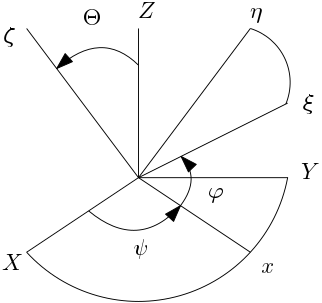
\includegraphics[width=5cm]{fig13.png} 
  \end{figure}  

  \begin{df} $ Ox = (OXY)\cap(O\xi\eta) $ - линия узлов \end{df}
  \begin{df} $\psi = \angle(Ox, OX)$ - угол прецессии \end{df}
  \begin{df} $\Theta = \angle (O\zeta, OZ)$ - угол нутации \end{df}
  \begin{df} $\varphi = \angle (Ox, O\xi)$ - угол собственного вращения \end{df}
  \begin{df} $\{\psi, \Theta, \varphi\}$ - углы Эйлера \end{df}

  Повороты:
  $ OXYZ \xrightarrow{\psi, OZ} OxyZ \xrightarrow{\Theta, Ox} Oxy\zeta \xrightarrow{\varphi, O\zeta} O\xi\eta\zeta $

  $\v{\omega} = \dot{\psi}\v{e}_Z + \dot{\Theta}\v{e}_x + \dot{\varphi}\v{e}_{\zeta}$

  $\v{e}_x = \cos \varphi \v{e}_{\xi} - \sin \varphi \v{e}_{\eta}$
  
  $\v{e}_z = \cos \Theta \v{e}_{\zeta} + \sin \Theta ( \sin \varphi \v{e}_{\xi} + \cos \varphi \v{e}_{\eta} )$
  $$\begin{array}{rcl}\v{\omega} & = & \dot\psi(\sin \Theta \sin \varphi \v{e}_{\xi} + \sin \Theta \cos \varphi \v{e}_{\eta} + \cos \Theta \v{e}_{\zeta}) \\
  & + & \dot \Theta (\cos \varphi \v{e}_{\xi} - \sin \varphi\v{e}_{\eta}) \\
  & + & \dot{\varphi}\v{e}_{\zeta} = \omega_{\xi}\v{e}_{\xi} + \omega_{\eta}\v{e}_{\eta} + \omega_{\zeta}\v{e}_{\zeta} \\
  \end{array}$$

  $$
  \begin{cases}
  \v{\omega}_{\xi} = \dot{\psi}\sin\Theta \sin\varphi + \dot{\Theta}\cos\varphi \\
  \v{\omega}_{\eta} = \dot{\psi}\sin\Theta \cos\varphi - \dot{\Theta}\sin\varphi \\
  \v{\omega}_{\zeta} = \dot{\psi}\cos\Theta + \dot{\varphi} \\
  \end{cases}
  \text{ - кинематические формулы Эйлера}
  $$

  \begin{df} 
  Движение твердого тела называется прецессией, если некоторая ось, неподвижная в теле, в абсолютном пространстве движется по поверхности неподвижного кругового конуса. $\dot{\Theta} = 0$. Если $\dot {\psi} = const$, $\dot {\varphi} = const$, то прецессия называется регулярной.
  \end{df}

  \section{Алгебра кватернионов}
  \begin{df} Алгеброй над полем называется векторное пространство над этим полем, снабженное билинейной операцией умножения. \end{df}
  \begin{xmp} ~

  $\underline{n=2}$(\textit{Комплексные числа}). $z_1 = a + bi$, $z_2 = c + di$ 

  $$ z_1z_2 = (ac - bd) + (ad + bc)i $$

  \end{xmp}
  $\underline{n=4}$(\textit{Алгебра кватернионов})

  \begin{flalign*}
  & \Lambda = \lambda_0 \v{i}_0 + \lambda_1 \v{i}_1 + \lambda_2 \v{i}_2 + \lambda_3 \v{i}_3 \in \mathbb{H} &\\
  & \{\v{i}_0, \v{i}_1, \v{i}_2, \v{i}_3\} \text{ - базис} &\\ 
  & \Lambda = \lambda_0 + \overline{\lambda} &\\
  & i_0 \circ i_k = i_k \quad k = \overline{1, 3},~ i_0 \circ i_0 = 1 &\\
  & i_k \circ i_m = -(i_k, i_m) + [i_k, i_m] \quad k, m \in \{1,2,3\}, \qquad  \text{В частности, $i_k \circ i_k = -1$}&\\
  & \overline{\lambda} \circ \overline{\mu} = (\lambda_1 \v{i}_1 + \lambda_2 \v{i}_2 + \lambda_3 \v{i}_3) \circ (\mu_1 \v{i}_1 + \mu_2 \v{i}_2 + \mu_3 \v{i}_3) = -(\overline{\lambda}, \overline{\mu}) + [\overline{\lambda}, \overline{\mu}] &\\
  & \Lambda \circ M = (\lambda + \overline{\lambda}) \circ (\mu + \overline{\mu}) = \lambda_0 \mu_0 + \lambda_0\overline{\mu} + \overline{\lambda}\mu_0 - (\overline{\lambda}, \overline{\mu}) + [\overline{\lambda}, \overline{\mu}] &\\
  \end{flalign*}
  \paragraph{Свойства:}
  \begin{enumerate}
    \item $(\Lambda \circ M) \circ N = \Lambda \circ (M \circ N)$
    \item $(\Lambda + M) \circ N = \Lambda \circ N + M \circ N $
    \item $\Lambda \circ M \neq M \circ \Lambda$
  \end{enumerate}

  \lline
  %2017-10-04
  \begin{df}
  \[ \overline{\Lambda} = \lambda_0 - \overline{\lambda} \]
  \end{df}
  \begin{ass}
  \[ \overline{\Lambda \circ M} = \overline{M} \circ \overline{\Lambda} \]
  \end{ass}
  \begin{proof}
  \[ \overline{\Lambda \circ M} = \lambda_0\mu_0 - (\overline\lambda, \overline\mu) - \lambda_0\overline\mu - \mu_0\overline\lambda - [\overline\lambda, \overline\mu] = \]
  \[ = (\mu_0 - \overline\mu) \circ (\lambda_0 - \overline\lambda) = \overline M \circ \overline \Lambda \]
  \end{proof}
  \begin{df}
  \[ \parallel \Lambda \parallel = \Lambda \circ \overline \Lambda = (\lambda_0 + \overline \lambda) \circ (\lambda_0 - \overline \lambda) = \lambda_0^2 + \overline \lambda^2 = \sum\limits_{k = 0}^3 \lambda_k^2 = | \Lambda |^2 \text{ - норма $\Lambda$ }\]
  \end{df}
  \begin{ass}
  \[ \parallel \Lambda \circ M \parallel = \norm{\Lambda} \cdot \norm{M} \]
  \end{ass}
  \begin{proof}
  \[ \norm{\Lambda \circ M} = (\Lambda \circ M) \circ (\overline{\Lambda \circ M}) = \Lambda \circ \underbrace{M \circ \overline M}_{\norm{M}}  \circ \overline \Lambda = \norm{M} \cdot \norm{\Lambda} \]
  \end{proof}
  \begin{df}
  \[ \Lambda^{-1} = \frac{\overline \Lambda}{\norm{\Lambda}},~ \norm \Lambda \neq 0 \]
  \end{df}
  \begin{ntc}
  \[ \Lambda \circ \frac{\overline{\Lambda}}{\norm{\Lambda}} = \frac{\overline \Lambda}{\norm \Lambda} \circ \Lambda = \frac{\norm \Lambda}{\norm \Lambda} = 1 \]
  \end{ntc}

  \paragraph*{Формула Муавра}
  \begin{flalign*}
  & \Lambda = \lambda_0 + \overline \lambda =  \abs \Lambda \lb \frac{\lambda_0}{\abs \Lambda} + \frac{\overline \lambda}{\abs \lambda } \frac{\abs {\overline \lambda}}{\abs \Lambda} \rb = \abs \Lambda \lb \cos \nu + \overline e \sin \nu \rb &\\
  & \overline e = \frac{\overline \lambda}{\abs {\overline \lambda}},~ \cos\nu = \frac{\lambda_0}{\abs{\Lambda}},~ \sin\nu = \frac{\abs{\overline \lambda}}{\abs{\Lambda}} &\\
  & \Lambda_1 = \abs{\Lambda_1}(\cos \nu_1 + \overline e \sin \nu_1) &\\
  & \Lambda_2 = \abs{\Lambda_2}(\cos \nu_2 + \overline e \sin \nu_2) &\\
  & \Lambda_1 \circ \Lambda_2 = \abs{\Lambda_1}\cdot\abs{\Lambda_2}(\cos\nu_1 \cos\nu_2 - \sin\nu_1\sin\nu_2(\overline e, \overline e) + \cos\nu_1\sin\nu_2 \overline e + &\\ 
  & + \cos\nu_2\sin\nu_1\overline e + \sin\nu_2\sin\nu_2[\overline e, \overline e]) = \abs{\Lambda_1}\abs{\Lambda_2} \cdot (\cos(\nu_1 + \nu_2) + \overline e \sin(\nu_1 + \nu_2)) &\\
  \end{flalign*}
  \[ \Lambda^k = \abs \Lambda^k \cdot (\cos k\nu + \overline e \sin k\nu) \text{ --- формула Муавра } \]
  \section{Задание ориентации твердого тела с помощью кватернионов}
  $E = \{\ea, \eb, \ec\}$ --- неподвижный базис \\
  $E' = \{\ea', \eb', \ec' \}$ --- связанный с телом
  \begin{teo}
  Произвольному положению твердого тела с неподвижной точкой соответствует нормированный кватернион, удовлетворяющий равенству:
  \[ \v{e}_i' = \Lambda \circ \v{e}_i \circ \overline \Lambda,~~ i = 1\ldots3  \]
  \end{teo}
  \begin{ntc}
  $\Lambda$ --- нормирован, если $\norm \Lambda = 1$
  \end{ntc}
  \begin{proof}~
  \begin{enumerate}
  \item Нормированность
  \[ \norm{\ei'} = \norm \Lambda \cdot \norm{\ei} \cdot \norm{\overline{\Lambda}} \Rightarrow 1 = \norm \Lambda \cdot 1 \cdot \norm \Lambda \Rightarrow \norm \Lambda = 1 \]
  \item Существование решения. $\Lambda = \lambda_0 + \overline \lambda$
  \begin{flalign*}
  & 
  \begin{cases} 
  \lambda_0^2 + \overline \lambda^2 = 1  \\
  \ei' \circ \Lambda = \Lambda \circ \ei \\
  \end{cases}
  &
  \begin{cases}
  \lambda_0^2 + \overline \lambda^2 = 1 \\
  \ei' \circ (\lambda_0 + \overline \lambda) = (\lambda_0 + \overline \lambda) \circ \ei \\
  \end{cases}
  \end{flalign*}
  \begin{flalign*}
  &
  \begin{cases}
  \lambda_0 \ei' - (\ei', \overline \lambda) + [\ei', \overline \lambda] = \lambda_0\ei' - (\lambda, \ei') + [\overline \lambda, \ei] \\
  \lambda_0^2 + \overline \lambda^2 = 1 \\
  \end{cases}
  &\\
  \end{flalign*}
  \begin{flalign*}
  & \begin{cases}
  \lambda_0^2 + \overline \lambda^2= 1  \\
  (\overline \lambda, \overline r_i) = 0 \\
  \lambda_0 \overline r_i - [\overline \lambda, \overline s_i] = 0 \\
  \end{cases}
  &
  \overline r_i = \ei' - \ei,~ \overline s_i = \ei' + \ei & ~~i = 1 \ldots 3
  &\\
  \end{flalign*}
  \begin{enumerate}
  \item 
  \begin{flalign*}
  & (\overline r_k, \overline s_k) = (\ek' - \ek, \ek' + \ek) = (\ek', \ek') - (\ek, \ek) = 0 &\\
  & (\overline r_k, \overline s_l) = (\ek' - \ek, \el' + \el) = (\ek', \el') + (\ek', \el) -  (\ek, \el') - (\ek, \el) = &\\
  & = -(\el' - \el, \ek' + \ek) = -(\overline s_k, \overline r_l),~ k \neq l &\\
  \end{flalign*}
  \item \label{two.o}
  \begin{flalign*}
  & (\overline r_1, \overline r_2, \overline r_3) = (\ea' - \ea, \eb' - \eb, \ec' - \ec) = (\ea', \eb', \ec') - (\ea, \eb, \ec) - &\\ 
  & - (\ea', \eb', \ec) + (\ea, \eb, \ec') =  1 - 1 - (\underbrace{[\ea', \eb']}_{\ec'}, \ec) + (\underbrace{[\ea, \eb]}_{\ec}, \ec') = 0 &\\
  \end{flalign*}
  \item 
  \begin{flalign*}
  & \overline r_1(\overline s_2, \overline r_3) + \overline r_2(\overline s_3, \overline r_1) + \overline r_3(\overline s_1, \overline r_2) &\\
  & \re{two.o} \Rightarrow c_1\v r_1 + c_2\v r_2 + c_3\v r_3 = 0 &\\
  & 
  \begin{cases}
  0 + c_2(\v s_1, \v r_2) - c_3(\v s_2, \v r_1) = 0 \\
  -c_1(\v s_1, \v r_2) + 0 + c_3(\v s_2, \v r_3) = 0 \\
  c_1(\v s_3, \v r_1) - c_2 (\v s_2, \v r_3) + 0 = 0 \\    
  \end{cases}
  &\\
  &
  \begin{cases}
  c_1 = (\v s_2, \v r_3) \\
  c_2 = (\v s_3, \v r_1) \\
  c_3 = (\v s_1, \v r_2) \\
  \end{cases}
  \begin{cases}
  \lambda_0^2 + \lambda^2 = 1 \\
  (\v r_k, \v \lambda) = 0 \\
  \lambda_0\v r_k + [\v s_k, \v \lambda] = 0 \\
  \end{cases}
  \begin{array}{c}
  (1) \\ (2) \\ (3) \\
  \end{array}
  &\\
  &
  (3) \Leftrightarrow
  \begin{cases}
  \lambda_0\v r_1 + [\v s_1, \alpha[\v r_1, \v r_2]] = 0 \\
  \lambda_0\v r_2 + [\v s_2, \alpha[\v r_1, \v r_2]] = 0 \\
  \lambda_0\v r_3 + [\v s_3, \alpha[\v r_1, \v r_2]] = 0 \\
  \end{cases}
  &\\
  &
  \begin{cases}
  \lambda_0 \v r_1 + \alpha \v r_1 (\v s_1, \v r_1) - 0 = 0 \\
  \lambda_0 \v r_2 + 0 - \alpha\v r_2(\v s_2, \v r_1) = 0 \\
  \lambda_0 \v r_3 + \alpha r_1(\v s_3, \v r_2) - \alpha r_2(\v s_3, \v r_1) = 0 \\
  \end{cases}
  &\\
  &
  \begin{cases}
  \lambda_0\v r_1 + \alpha\v r_1(\v s_1,\v r_2) = 0 \\
  \lambda_0\v r_2 + \alpha\v r_2(\v s_1,\v r_2) = 0 \\
  \lambda_0\v r_3 + \alpha\v r_3(\v s_1,\v r_2) = 0 \\
  \end{cases}
  &
  \lambda_0 = -\alpha(\v s_1, \v r_2) = \alpha(\v s_2, \v r_1)
  &\\
  &
  (1) \Rightarrow \alpha^2((\v s_2, \v r_1)^2 + [\v r_1, \v e_2]^2)^2 = 1 \Rightarrow & \alpha = \pm \frac{1}{\sqrt{(\v s_2, \v r_1)^2 + [\v r_1, \v r_2]^2}} 
  &\\
  \end{flalign*}
  \[ \Lambda = \pm \frac{(\v s_2, \v r_1) + [\v r_1, \v r_2]}{\sqrt{(\v s_2, \v r_1)^2 + [\v r_1, \v r_2]^2}} \]
  \end{enumerate}
  \end{enumerate}
  \end{proof}
  \begin{df}
  \[ f(M) = \Lambda \circ M \circ \overline \Lambda;~~ M \rightarrow f(M),~~ \norm{\Lambda} = 1 \text{--- присоединенное преобразование} \]
  \end{df}
  \begin{ass}
  Присоединенное преобразование не меняет скалярные части кватернионов и модуль векторной части
  \end{ass}
  \begin{proof}~
  \begin{enumerate}
  \item
  $ f(M) = \Lambda \circ (\mu_0 + \overline \mu) \circ \overline \Lambda = \Lambda \circ \mu_0 \circ \overline \Lambda + \Lambda \circ \overline \mu \circ \Lambda = \mu_0 \norm \Lambda + f(\v \mu) = \mu_0 + \v \mu ' $
  \item $\mu_0^2 + \v \mu^2 = \norm M = \norm{\Lambda \circ M \circ \v \Lambda} = \norm{f(M)} = \mu_0^2 + \v \mu'^2 \Rightarrow \mu^2 = \v \mu'^2$
  \end{enumerate}
  \end{proof}
  \begin{cor}
  Всегда существует присоединенное преобразование, переводящее орты неподвижного базиса в орты базиса, связанного с телом.
  \end{cor}
  \begin{proof}
  \begin{flalign}
  & \ei' = \Lambda \circ \ei \circ \v \Lambda = f(\ei) &\\
  & \v r = \sum\limits_{k = 1}^3 r_k \ek,~~ f(r) = \Lambda \circ \sum r_k \ek \v \Lambda = \sum\limits_k r_k f(\ek) = \sum\limits_k = r_k\ek = \v r ' &\\
  \end{flalign}
  \end{proof}
  \begin{equation}
  \label{b.star}
  \boxed{\v r' = \Lambda \circ \v r \circ \v \Lambda}
  \end{equation}
  \begin{cor}
  При повороте твердого тела вокруг неподвижной точки справедлива \re{b.star}, где $\v r$ -- начальное положение точки, $\v r'$ -- ее положение после поворота, а $\Lambda$ -- кватернион соответствующего преобразования.
  \end{cor}